\begin{question}
  \hspace*{\fill} [Note Maximale: ?]\par
  \begin{center} % or flushleft or flushright
    \noindent La représentation graphique dune fonction $f$ est tracée sur la figure ci-dessous.\par
    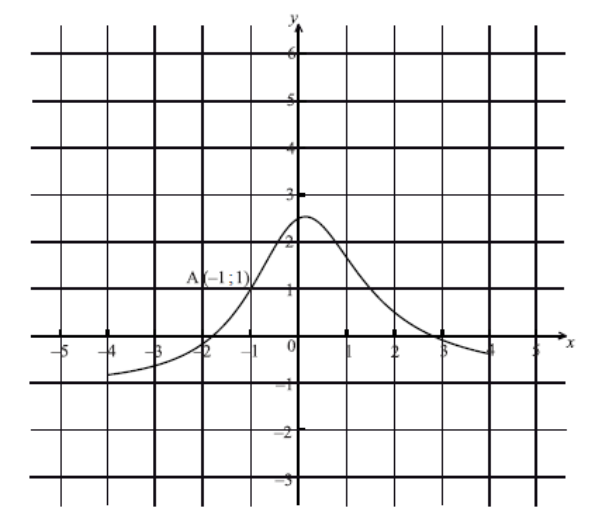
\includegraphics[scale=0.3]{figure_x17}\par
    \noindent Le point $A(-1; 1)$ est sur la représentation graphique. et $y=-1$ est un asymptote horizontale.\par
  \end{center} % or flushleft or flushright
  \begin{enumerate}[label=(\alph*)]
    \item Soit $g(x) = f(x-1) + 2$. Sur la figure esquissez la représentation graphique de $g$.\hspace*{\fill} [?]
    \item Donnez l'équation de l'asymptote de $g$.\hspace*{\fill} [?]
    \item Soit $A^\prime$ le point sur la représentation graphique de $g$ correspondant au point $A$.  Donnez les coordonnées de $A^\prime$.\hspace*{\fill} [?]
  \end{enumerate}
\end{question}
